% Chapter Template

\chapter{Memoria de Reconocimiento} % Main chapter title

\label{Cap_RM} % Change X to a consecutive number; for referencing this chapter elsewhere, use \ref{ChapterX}

%----------------------------------------------------------------------------------------
%	SECTION 1
%----------------------------------------------------------------------------------------
En este capítulo se revisará 

\section{Modelos utilizados en el estudio de la Memoria de Reconocimiento}

\subsection{Teoría del Umbral}

Lorem ipsum dolor sit amet, consectetur adipiscing elit. Aliquam ultricies lacinia euismod. Nam tempus risus in dolor rhoncus in interdum enim tincidunt. Donec vel nunc neque. In condimentum ullamcorper quam non consequat. Fusce sagittis tempor feugiat. Fusce magna erat, molestie eu convallis ut, tempus sed arcu. Quisque molestie, ante a tincidunt ullamcorper, sapien enim dignissim lacus, in semper nibh erat lobortis purus. Integer dapibus ligula ac risus convallis pellentesque.

%-----------------------------------
%	SUBSECTION 1
%-----------------------------------
\subsection{Teoría del Procesamiento Dual}

La Teoría del Procesamiento Dual (TPD; o PDT por sus siglas en inglés) sostiene que existen dos procesos fundamentales involucrados en todo juicio de reconocimiento: la recolección y el análisis de familiaridad. El primero corresponde a la extracción de rasgos y detalles específicos del estímulo a evaluar, (i.e. el estímulo que queremos determinar si se ha visto antes, o no), un proceso que requiere cierto tiempo; el segundo, es entendido como un fenómeno más o menos automático y casi instantáneo donde el sistema identifica el estímulo como 'familiar' y decide que lo ha reconocido de alguna experiencia previa. 

Lorem ipsum dolor sit amet, consectetur adipiscing elit. Aliquam ultricies lacinia euismod. Nam tempus risus in dolor rhoncus in interdum enim tincidunt. Donec vel nunc neque. In condimentum ullamcorper quam non consequat. Fusce sagittis tempor feugiat. Fusce magna erat, molestie eu convallis ut, tempus sed arcu. Quisque molestie, ante a tincidunt ullamcorper, sapien enim dignissim lacus, in semper nibh erat lobortis purus. Integer dapibus ligula ac risus convallis 
pellentesque.

Lorem ipsum dolor sit amet, consectetur adipiscing elit. Aliquam ultricies lacinia euismod. Nam tempus risus in dolor rhoncus in interdum enim tincidunt. Donec vel nunc neque. In condimentum ullamcorper quam non consequat. Fusce sagittis tempor feugiat. Fusce magna erat, molestie eu convallis ut, tempus sed arcu. Quisque molestie, ante a tincidunt ullamcorper, sapien enim dignissim lacus, in semper nibh erat lobortis purus. Integer dapibus ligula ac risus convallis pellentesque.
%-----------------------------------
%	SUBSECTION 2
%-----------------------------------

\subsection{Teoría de Detección de Señales}
Aplicar la TDS al estudio de la Memoria de Reconocimiento implica asumir que existe tal cosa como una 'fuerza de memoria' ('memory strength', en inglés) que refleja el grado en que un estímulo cualquiera es percibido como 'familiar' para el sistema que busca emitir un juicio de detección. La fuerza de memoria evocada por cada estímulo se compara con un criterio de elección para que el sistema pueda decidir si lo reconoce, o no, como 'elemento antes visto'.\\ 

\begin{figure}[th]
\centering
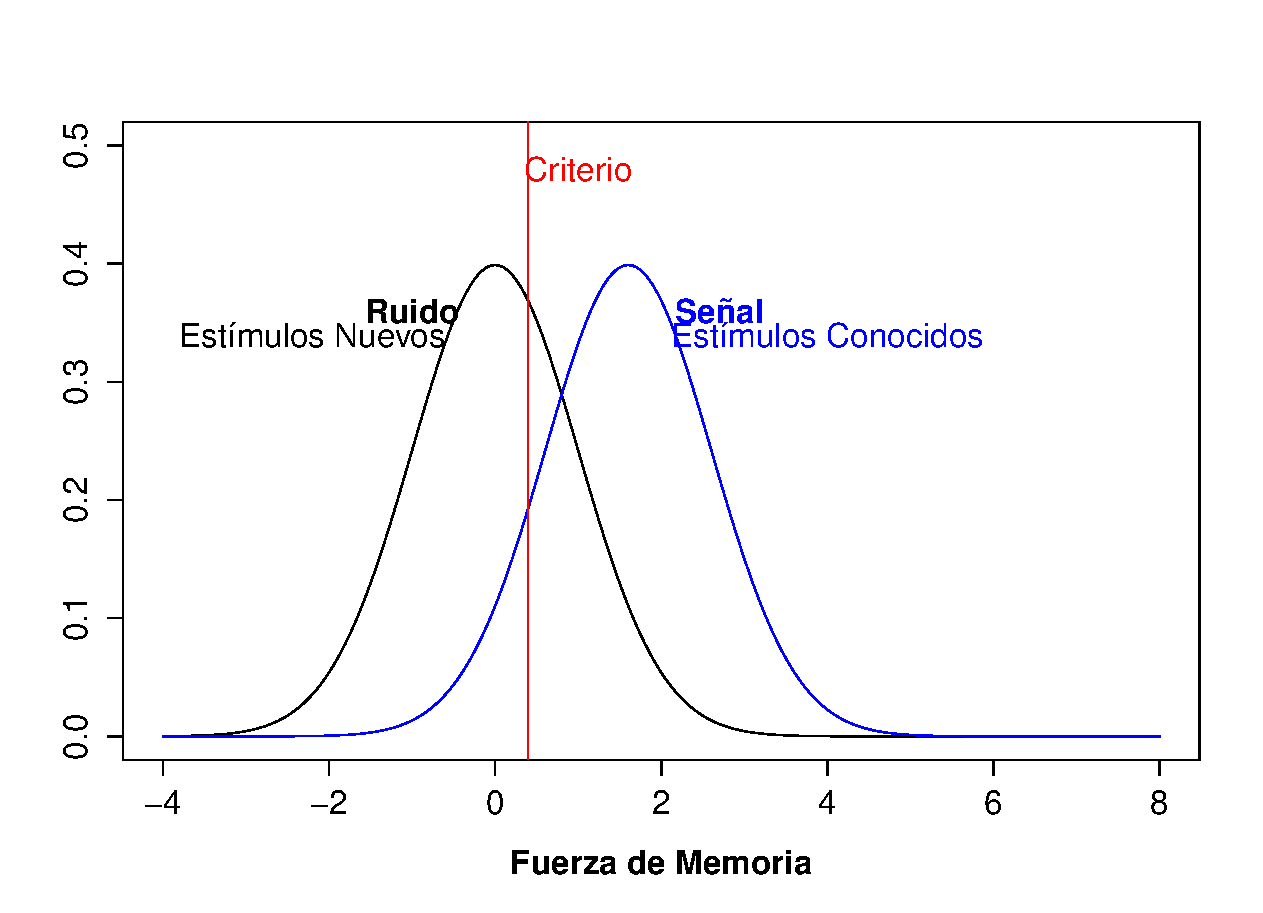
\includegraphics[width=0.60\textwidth]{Figures/RM_SDT_1} 
\decoRule
\caption[SDT en Memoria de Reconocimiento]{Modelo de Detección de Señales aplicado al estudio de Memoria de Reconocimiento}
\label{fig:RM_SDT_1}
\end{figure}

La Figura~\ref{fig:RM_SDT_1} ilustra la forma en que los supuestos de la TDS, expuestos a detalle en el Capítulo 1, se aplican al estudio de la Memoria de Reconocimiento. Las idea central se mantiene en escencia y simplemente sustituimos algunos conceptos: al tratarse de una tarea de reconocimiento, decimos que la 'señal' a detectar es cualquier estímulo antes visto (i.e. 'estímulos viejos', como suelen identificarse en la literatura); el 'ruido' son los estímulos nuevos, que podrían -o no- confundirse con los primeros; el 'eje de decisión' a lo largo del cual se sitúan las dos distribuciones de ruido y señal, se convierte en un 'eje de familiaridad' que va a representar distintos grados de lo que parece ser una 'fuerza de memoria'. También se mantienen las ideas centrales propuestas por el modelo: los estímulos ya antes vistos tendrán valores más altos de 'familiaridad' que aquellos nunca antes vistos, admitiendo sin embargo la posibilidad de que éstos últimos puedan llegar a confundirse con los estímulos viejos, por ejemplo, si comparten algun rasgo en particular; una vez más, dicha variabilidad en la presentación y lectura de los estímulos a evaluar se refleja en la idea de que existen distintos rangos de familiaridad que pueden ser producidos por los estímulos viejos o conocidos, con cierta distribución de probabilidad. Y de la misma forma, la emisión de un juicio se entiende como resultado de comparar la 'familiaridad' de cada estímulo a evaluar con un criterio de elección particular, donde sólo si éste se rebasa, se juzga el estímulo como 'ya antes visto'.\\

Como se mencionó en el Capítulo 1, la TDS en su forma típica define las distribuciones de ruido y señal como distribuciones Gaussianas con varianzas iguales (i.e. con una misma desviación estándar). A propósito de ello, podemos hablar de una particularidad que tiene la aplicaicón de la TDS a estudios de memoria de reconocimiento, que ha sido constante y consistentemente demostrada con los datos: la distribución de Estímulos Viejos suele mostrar mayor desviación estándar que la distribución de Ruido, justo como se muestra en la Figura~\ref{fig:RM_SDT_2}.\\


\begin{figure}[th]
\centering
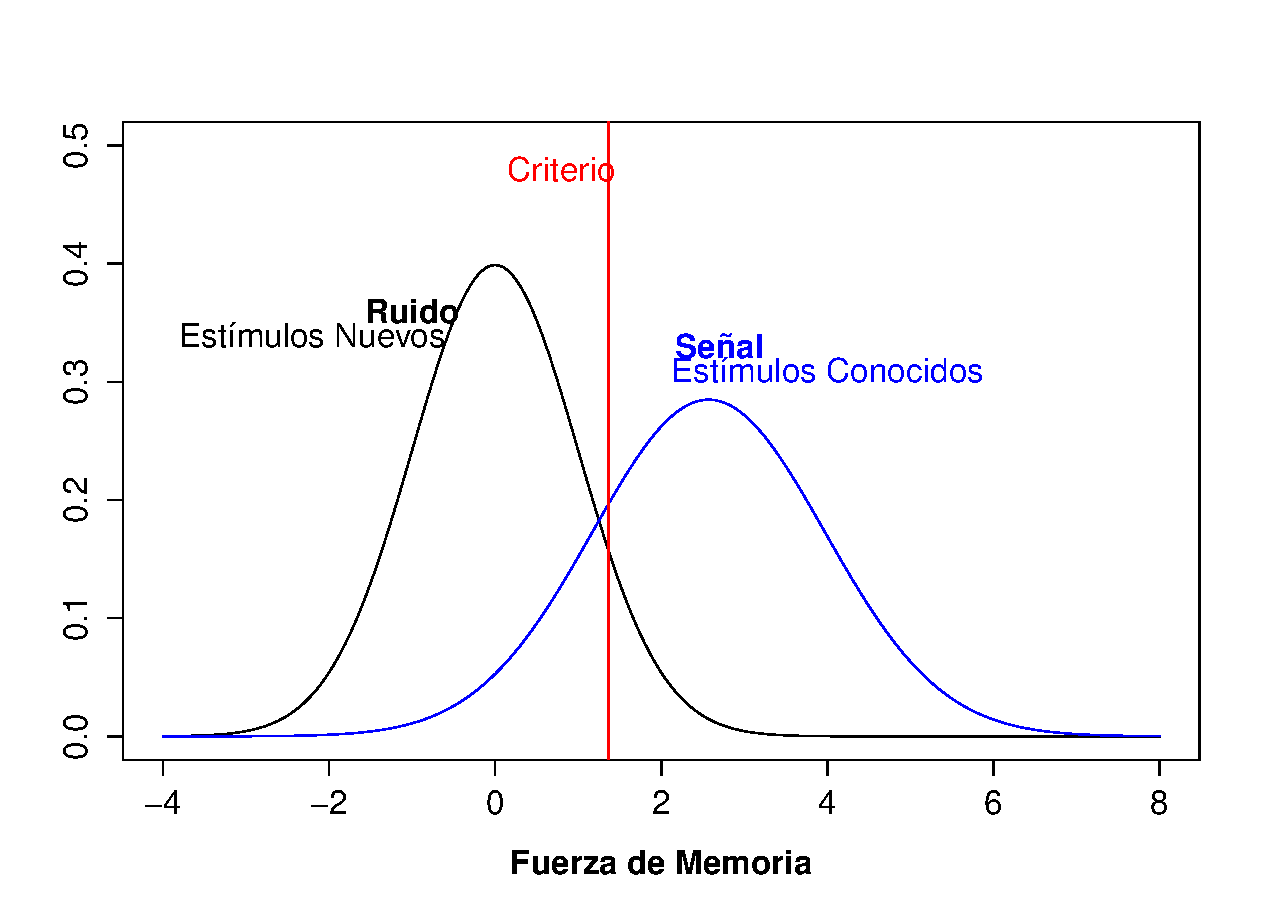
\includegraphics[width=0.60\textwidth]{Figures/RM_SDT_2} 
\decoRule
\caption[SDT en Memoria de Reconocimiento (Varianzas Desiguales)]{Modelo de Detección de Señales con varianzas desiguales aplicado al estudio de Memoria de Reconocimiento}
\label{fig:RM_SDT_2}
\end{figure}


\section{Conflicto entre modelos}

Me permitiré, por un momento, salirme del molde académico y hablar un poco de todo el proceso que hubo detrás de la realización del presente trabajo. Cuando comencé a revisar literatura para decidir cuál podría ser mi proyecto de tesis, descubrí la maravilla de la Teoría de Detección de Señales. 

Sin embargo, pese a la flexibilidad de la que dispone la TDS para aplicarse a, aparentemente, cualquier tarea de decisión binaria, donde se admita el papel de la incertidumbre en la emisión de un juicio de detección, su aplicación al campo de la Memoria de Reconocimiento no ha estado excenta de críticas.

Conceptualmente, es fácil pensar en una tarea de reconocimiento en términos del modelo de detección de señales. Sin embargo, cuando se revisan las implicaciones teóricas que conllevaría aceptar que la memoria de Reconocimiento funciona como un procedimiento cualquiera de detección de señales, no son del todo claras. 

\subsection{Proceso Dual Detección de Señales - Umbral alto}

Ante el conflicto existen siempre distintos caminos y estilos de afrontamiento. La TDS ha sido vista como antagonista directa de los modelos de Procesamiento Dual en tanto que define el problema del reconocimiento como dependiente de un sólo proceso de comparación de la familiaridad percibida con un criterio de elección del sistema. Existe una amplia literatura, que discutiremos más adelante, que se ha enfocado en poner a prueba dichos modelos para comparar directamente su poder.

Una estrategia diferente para resolver este conflicto entre la TDS y el Procesamiento Dual es hacer a un lado la recolección de evidencia que pudiera otorgar a uno de los dos enfoques en competencia la victoria definitiva para concentrarse en la conciliación de estos modelos, ya sea desde el plano conceptual, o bien, a partir del desarrollo de un nuevo modelo unificador.

Por ejemplo, en una serie de experimentos presentados por \parencite{Atkinson1973}, 



\subsection{}

Una vía alterna para solucionar el conflcitoque se tiene con 







%----------------------------------------------------------------------------------------
%	SECTION 2
%----------------------------------------------------------------------------------------

\section{El Efecto Espejo}


